\Chapter{A Vue alkalmazás működése}

Az elkészített alkalmazás működésének megértéséhez szükséges először a \textit{Vue} keretrendszer alapvető elemeit, fogalmait megnézni.

\Section{A \textit{Vue.js} bemutatása}

A \textit{Vue.js} egy JavaScript keretrendszer, melynek fejlesztését Evan You kezdte el, és 2014-ben jelent meg először. Célja az volt, hogy egy könnyű keretrendszert készítsen az Angular előnyeinek megtartásával. A \textit{Vue.js} egy MVC-hez hasonló architektúrát követ. Adataink, függvényeink, illetve a HTML megjelenítés remekül szétválasztható, ami miatt összességében egy átláthatóbb kódot kapunk eredményül. Egy \textit{Vue} alkalmazás komponensekből épül fel, melyek akár többször is felhasználhatók ugyanazon alkalmazás részeként (\ref{fig:components}. ábra).

\begin{figure}[h!]
\centering
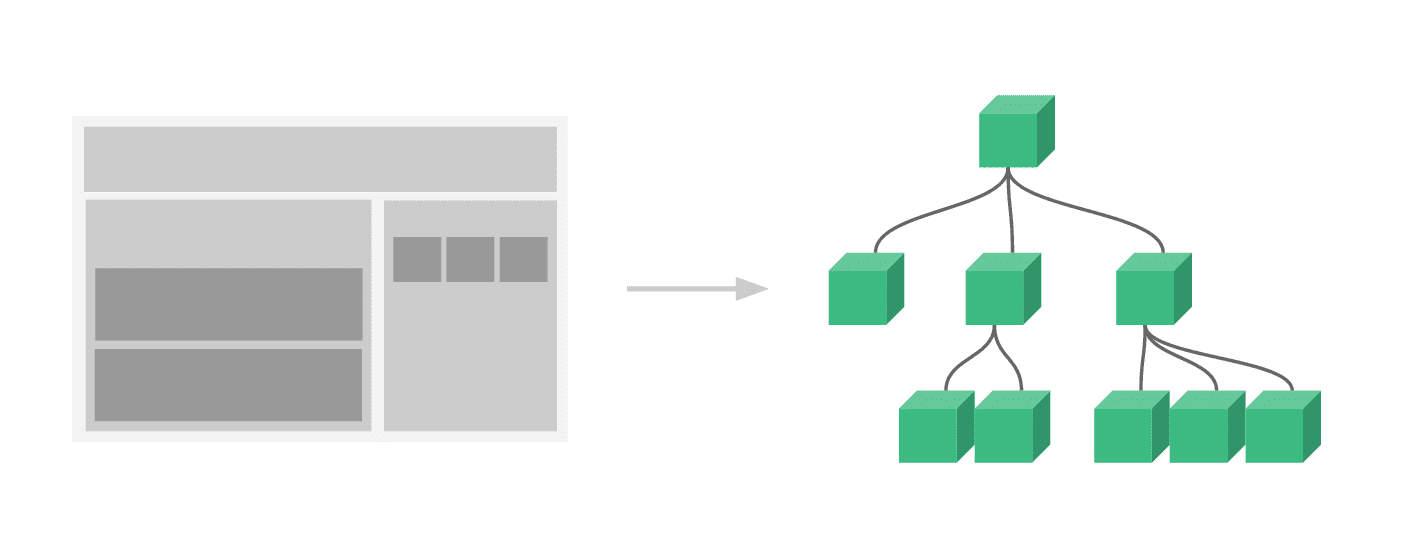
\includegraphics[scale=0.3]{images/components.png}
\caption{VueJS komponens kapcsolatok, forrás: \url{https://vuejs.org}.}
\label{fig:components}
\end{figure}

A következő szakaszokban nézzük is meg egy \textit{Vue} projekt megvalósítást, komponensekkel együtt, lépésenként.

\subsection{Projekt létrehozása}

Egy \textit{Vue} projekt létrehozásához egyaránt használhatunk parancsoros vagy grafikus felülettel rendelkező \textit{wizard}-ot. A következő lépések a grafikus felülettel történő projekt létrehozást mutatják be.
\begin{enumerate}
  \item Nyitunk egy terminált, majd beírjuk a következő parancsot: \texttt{vue ui}
  A parancs beírását követően egy projekt kezelő nyílik meg a böngészőnkben (\ref{fig:vueui}. ábra).
  
  \begin{figure}[h!]
  	\centering
  	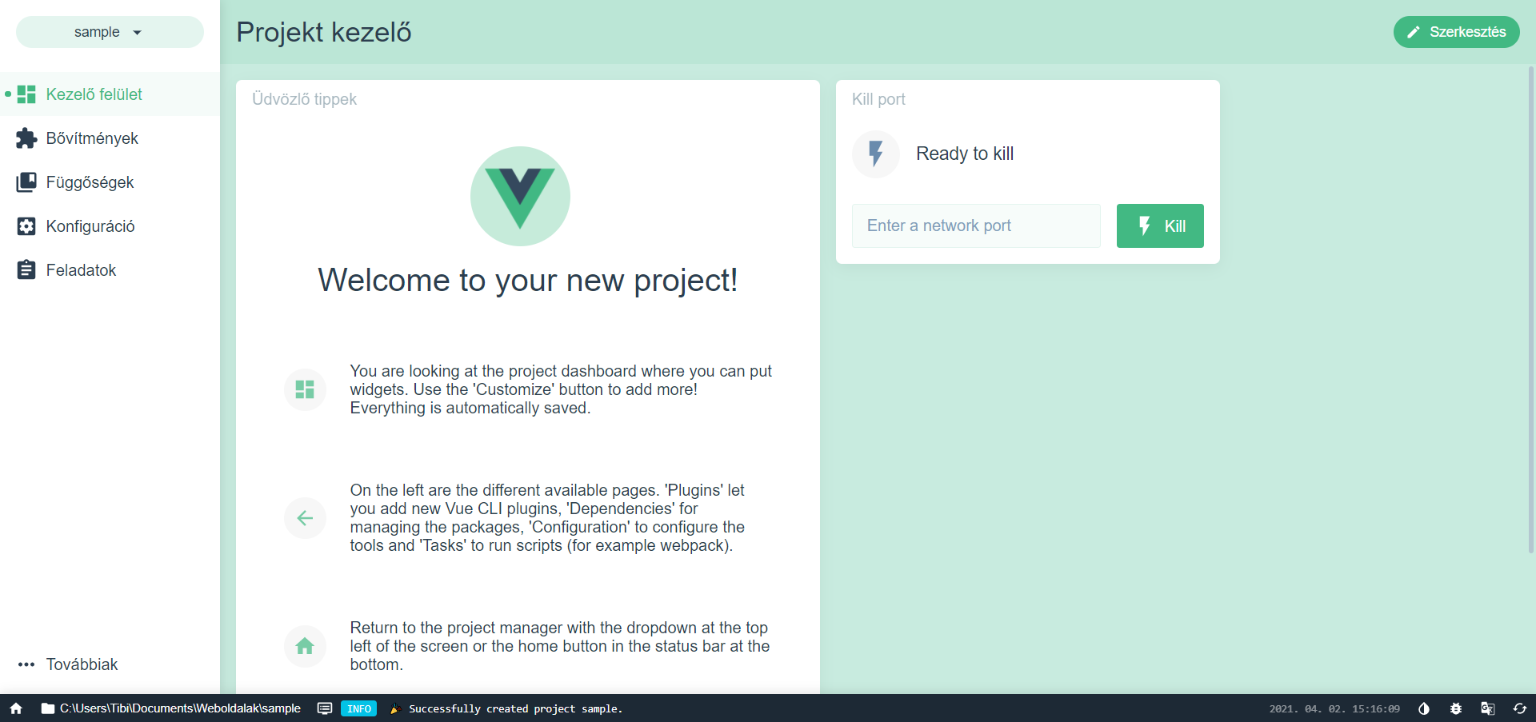
\includegraphics[width=\textwidth]{images/1617369552704.png}
  	\caption{\textit{VueJS} projekt kezelő}
  	\label{fig:vueui}
  \end{figure}

  \item Kattintsunk a “Továbbiak” gombra, majd a “Vue projekt kezelő”-re.
  \item Nyissuk meg a “Létrehozás” fület, majd válasszuk ki, hogy hova szeretnénk létrehozni az új vue projektünket.

  \item Nevezzük el a projektet, majd kattintsunk a “Következő” gombra.

  \item Válasszuk ki, hogy melyik Vue verziót szeretnénk alkalmazni (\ref{fig:vueversion}. ábra). Ebben a példában a Vue 2-t fogom választani. Ha készen vagyunk, kattintsunk a “Create" gombra.
  
\begin{figure}[h!]
\centering
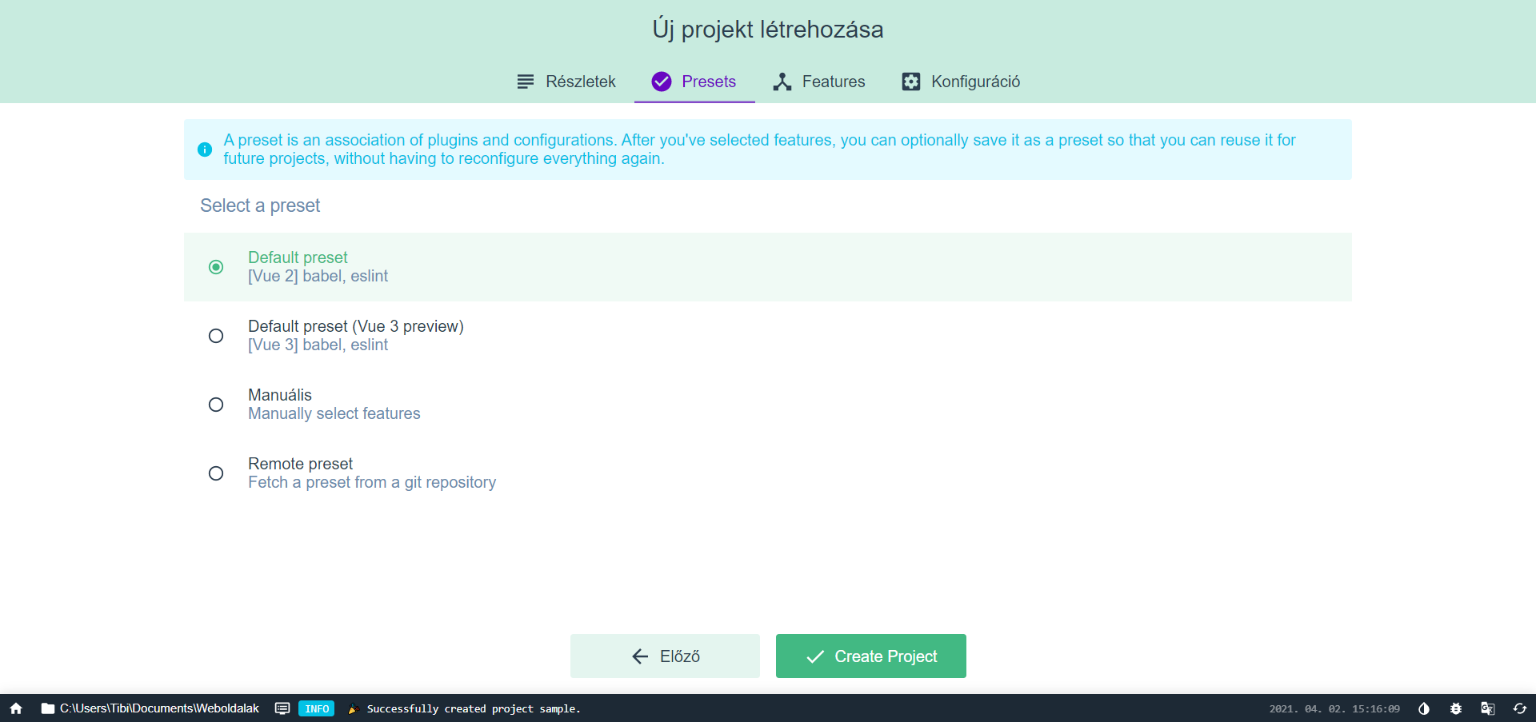
\includegraphics[width=\textwidth]{images/1617369965789.png}
\caption{Verzió kiválasztása}
\label{fig:vueversion}
\end{figure}

\item A projektünk mappájában nyissunk meg egy terminált, majd írjuk be a következő parancsot: \texttt{npm run serve}
\item Ha minden sikeres volt, nyissuk meg a böngészőben a \texttt{localhost:8080} URL-t. Ekkor \aref{fig:vueready}. ábrán látható kép fog minket fogadni.
 
\begin{figure}[h!]
\centering
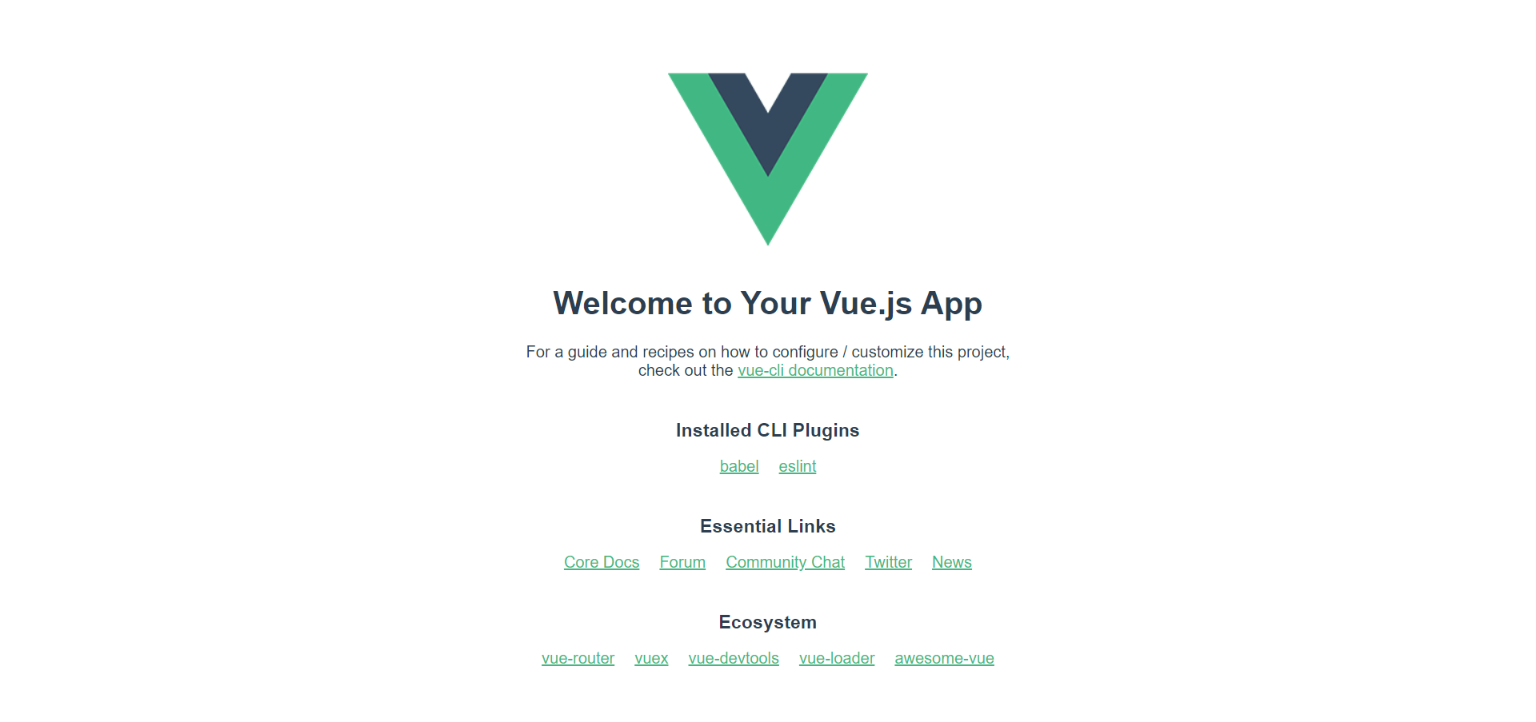
\includegraphics[width=\textwidth]{images/1617370382875.png}
\caption{Kész projekt}
\label{fig:vueready}
\end{figure}

\end{enumerate}

\subsection{Komponens hozzáadása}

\begin{enumerate}
	\item A projekt létrehozása során automatikusan generált nekünk a components mappán belül egy \texttt{HelloWorld.vue} nevű fájlt. Ebben a mappában érdemes tárolni más komponenseket is, a rendezettség és áttekinthetőség miatt. Ebből a fájlból kitörlöm azokat a részeket, amik a példába nem töltenek be szerepet (\ref{fig:hello}. ábra).
	
	\begin{figure}[h!]
	\centering
	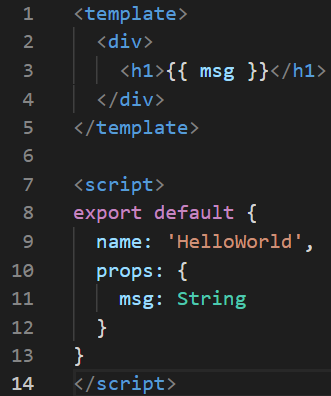
\includegraphics[scale=0.5]{images/14dfb7fd47c01c0cd6d8692ca740c349.png}
	\caption{Minta komponens kódja}
	\label{fig:hello}
	\end{figure}

	\begin{itemize}
		\item A \texttt{<template></template>} tagek között a HTML megjelenés található,
		\item \texttt{name} -- a komponens elnevezése,
		\item \texttt{props} -- Ez egy tömb, melynek több adata is lehet, ezeket az értékeket várja az \texttt{App.vue}-tól.
	\end{itemize}
	\item Az \texttt{App.vue}-hoz, most hozzáadjuk a \texttt{HelloWorld.vue} komponenst. Ezt úgy tudjuk megtenni, hogy a \texttt{<script></script>} tagek között importáljuk a fájlt.
\begin{javascript}
import HelloWorld from './components/HelloWorld.vue'
\end{javascript}
	Illetve a “components” tagjához is hozzáadjuk:
\begin{javascript}
components: {
  HelloWorld
}
\end{javascript}

 \item Nincs más dolgunk, mint alkalmazni a <template></template> tagek között. Ahhoz, hogy bemutassam, hogy egy komponenst kétszer is lehet használni különböző adatokkal ugyanabban az alkalmazásban a következőként fogom alkalmazni:

\begin{verbatim}
<HelloWorld msg="Én vagyok az első komponens"/>
<HelloWorld msg="Ugyanolyan komponens vagyok, csak más értékkel"/>
\end{verbatim}
\Aref{fig:result}. ábrán látható az eredmény.
\begin{figure}[h!]
	\centering
	
\includegraphics[scale=0.25]{images/1617372108829.png}
	\caption{Példa megjelenítése}
	\label{fig:result}
	\end{figure}
\end{enumerate}

\Section{Változók}

Az alkalmazás a következő változókat használja.

\begin{itemize}
	\item \texttt{socket: {}} -- Szerverhez való kapcsolódáshoz szükséges,
	\item \texttt{name: 'Anonymus'} -- Játékos neve,
	\item \texttt{skin: null} -- Játékos kinézete,
	\item \texttt{status: 'connecting'} -- Játékos aktuális státusza,
	\item \texttt{ingame: false} -- Játékban való részvétel,
	\item \texttt{isActive: false} -- Éppen a játékos van-e soron az adott körben,
	\item \texttt{isBuying: false} -- Megvásárolható ingatlanon áll-e a játékos,
	\item \texttt{isInventoryCheck: false} -- Nézi-e valaki inventory-át a játékos,
	\item \texttt{isSellCheck: false} -- Az Eladás menüpontban van-e a játékos,
	\item \texttt{isUpgradeCheck: false} -- A Fejlesztés menüpontban van-e a játékos,
	\item \texttt{isDestroyCheck: false} -- A Bontás menüpontban van-e a játékos,
	\item \texttt{isTradeCheck: false} -- A Csere menüpontban van-e a játékos,
	\item \texttt{tradeStatus: 0} -- A játékos státusza az aktuális cserében,
	\item \texttt{isTrading: false} -- A játékos éppen kereskedik-e,
	\item \texttt{tradeWindow: null} -- A kereskedésben megadott információkat tárolja,
	\item \texttt{inventoryCheckName: ''} -- Játékos neve akinek az inventory-át éppen nézi,
	\item \texttt{skins: []} -- Tárolja a beolvasott kinézeteket,
	\item \texttt{cards: []} -- Tárolja a beolvasott kártyákat,
	\item \texttt{messages: []} -- Tárolja a szervertől kapott üzeneteket,
	\item \texttt{jailtime: null} -- Játékos aktuális börtönideje,
	\item \texttt{freecard: 0} -- Játékos aktuális ingyen szabadulhatsz a börtönből kártyái,
	\item \texttt{money: 0} -- Játékos aktuális pénze,
	\item \texttt{doubleDice: 0} -- Hányszor dobott a játékos mióta ő van körön (dupla illetve tripla dobások miatt szükséges),
	\item \texttt{game: new Game()} -- Aktuális játék állása.
\end{itemize}

\Section{Kommunikáció a szerverrel}

Abban az esetben, hogyha kérést szeretnénk indítani a szerver felé, a
\begin{javascript}
this.socket.emit('sendmessageSocket', {
	msg: data, sender: this.name
});
\end{javascript}
függvényt kell alkalmaznunk. A '\texttt{sendmessageSocket}' lesz a kérés, a 
\begin{javascript}
{msg: data, sender: this.name}
\end{javascript}
pedig az objektum, amit küldeni szeretnénk. Ez természetesen lehet egy egyszerű érték is. A szerver ezt a
\begin{javascript}
socket.on('sendmessageSocket', (data) => {
  // ...
}
\end{javascript}

függvénnyel kezeli le. Fordített esetben, ha a szerver szeretne utasítást küldeni a kliensnek, ezt megteheti a
\begin{javascript}
io.emit('sendmessageFromSocket', (messages));
\end{javascript}
illetve
\begin{javascript}
socket.emit('sendmessageFromSocket', (messages));
\end{javascript}
függvényekkel is. A különbség közöttük, hogy az io.emit az összes szerveren lévő kliensnek kiküldi ezt az utasítást, a socket.emit viszont csak az éppen aktuális kliensnek, aki kérést intézett a szerver felé.

\subsection{Kérés küldése komponensből}

Esetemben több olyan alkalomra is sor került, amikor egy vue komponensből kellett kérést küldenem a szerver felé. Általában ezt úgy szokták megoldani egy vue alkalamzásban, hogy először az App.vue-ba emitelnek a következő módon:
\begin{javascript}
this.$emit('sendmsg',(this.cMsg));
\end{javascript}%$
Az \texttt{App.vue}-nak ezután ezt lekell kezelnie.
\begin{verbatim}
<Chat @sendmsg="getMessage(\$event)" … />
\end{verbatim}%$
Láthatjuk, hogy a Chat komponensből érkezett a kérés sendmsg néven. Ennek hatására lefut a getMessage funkció az \texttt{App.vue}-ban:
\begin{javascript}
getMessage(data){
  this.socket.emit('sendmessageSocket', {
    msg: data, sender: this.name
  });
}
\end{javascript}
Ez a függvény tovább küldi a szervernek egy kérést, illetve vele együtt a kapott adatokat.

\Section{Komponensek}

Az alkalmazás az alábbi komponensekből épül fel.

\begin{itemize}
	\item \texttt{OnlinePlayers} - Játékosok adatainak megjelenítésére szolgáló felület.
	\item \texttt{Login} - Bejelentkező felület.
	\item \texttt{Waiting} - Várakozó felület.
	\item \texttt{Table} - Játéktábla, emellett a használható gombok is ezen a komponensen belül található.
	\item \texttt{Chat} - Kommunikációs felület.
	\item \texttt{Inventory} - Az aktuálisan kiválasztott játékos megvásárolt bizniszeit/szolgáltatóit/telkeit jeleníti meg.
	\item \texttt{Sell} - Értékek eladására szolgáló felület.
	\item \texttt{Upgrade} - Telkek fejlesztésére szolgáló felület.
	\item \texttt{Destroy} - Telkek bontására alkalmas felület.
	\item \texttt{Trade} - Ebben a komponensben lehet kezdeményezni egy kereskedést.
	\item \texttt{TradePartner} - Hasonló a Trade komponenshez, viszont ez a másik fél szemszögében jelenik meg.
\end{itemize}
